% !TeX program = xelatex
% !TeX encoding = UTF-8
% !TeX spellcheck = en_US
% !BIB program = bibtex
%%
%% The above lines help editors like TeXstudio to automatically choose the right tools
%% to compile your LaTeX source file.
%%
%%%%%%%%%%%%%%%%%%%%%%%%%%%%%%%%%%%%%%%%%%%%%%%%%%%%%%%%%%%%%%%%%%%%%%%%%%%%%%%%

%%%%%%%%%%%%%%%%%%%%%%%%%%%%%%%%%%%%%%%%%%%%%%%%%%%%%%%%%%%%%%%%%%%%%%%%%%%%%%%%
%%
%%            JJJJ   K                         K   UUUU         UUUU
%%            JJJJ   KKKK                   KKKK   UUUU         UUUU
%%            JJJJ   KKKKKK               KKKKKK   UUUU         UUUU
%%            JJJJ      KKKKKK         KKKKKK      UUUU         UUUU
%%            JJJJ         KKKKKK   KKKKKK         UUUU         UUUU
%%            JJJJ            KKKKKKKKK            UUUU         UUUU
%%    JJ     JJJJJ               KKK               UUUUU       UUUUU
%%  JJJJJJJJJJJJJ    KKKKKKKKKKKKKKKKKKKKKKKKKKK    UUUUUUUUUUUUUUU
%%    JJJJJJJJJ      KKKKKKKKKKKKKKKKKKKKKKKKKKK      UUUUUUUUUUU
%%
%% This is an example file for using the JKU LaTeX technical report template.
%%
%%%%%%%%%%%%%%%%%%%%%%%%%%%%%%%%%%%%%%%%%%%%%%%%%%%%%%%%%%%%%%%%%%%%%%%%%%%%%%%%

\documentclass[a4paper,oneside,10pt,ngerman,english]{scrartcl}

\usepackage[utf8]{inputenc}

%%
%% Use the JKU LaTeX technical report template for this document.
%%
\usepackage[techreport,fancyfonts]{jkureport}

%%%%%%%%%%%%%%%%%%%%%%%%%%%%%%%%%%%%%%%%%%%%%%%%%%%%%%%%%%%%%%%%%%%%%%%%%%%%%%%%
%%
%% LOAD PACKAGES
%%

%% Replaced biblatex with natbib and specific style settings per your request
\usepackage{natbib}
\setcitestyle{authoryear,round,citesep={;},aysep={,},yysep={;}}

\usepackage{todonotes}
\usepackage{import}
\usepackage{amsfonts}
\usepackage{subfigure}
\usepackage{acronym}

%%
%%%%%%%%%%%%%%%%%%%%%%%%%%%%%%%%%%%%%%%%%%%%%%%%%%%%%%%%%%%%%%%%%%%%%%%%%%%%%%%%


\begin{document}
%%%%%%%%%%%%%%%%%%%%%%%%%%%%%%%%%%%%%%%%%%%%%%%%%%%%%%%%%%%%%%%%%%%%%%%%%%%%%%%%
%%
%% Report information and title page
%%

\title{Space for your report title}

\subtitle{Technical Report\\%
	\usekomafont{subtitlesmall}%
	\hfill\\%
	Optional space for mentioning e.g.\ your research lab\\
	\hfill\\%
}

\author{%
	Firstname1 Lastname1 \and Firstname2 Lastname2 \and Firstname3 Lastname3
	\affiliation{Institute of Networks~and~Security}
	\authornewline
	\authorphone{+43 732 2468-XXXX}
	\authormail{firstname.lastname@jku.at}
	\authorweb{https://jku.at/ins}
	\authornewline
}

\revisionblock{Space for your revision block, acknowledgements, etc.}

\abstract{Space for your (short) abstract.}

\maketitle
%%
%%%%%%%%%%%%%%%%%%%%%%%%%%%%%%%%%%%%%%%%%%%%%%%%%%%%%%%%%%%%%%%%%%%%%%%%%%%%%%%%

%%%%%%%%%%%%%%%%%%%%%%%%%%%%%%%%%%%%%%%%%%%%%%%%%%%%%%%%%%%%%%%%%%%%%%%%%%%%%%%%
%%
%% Add a table of contents
%%

\cleardoubleoddpage
\tableofcontents

%%
%%%%%%%%%%%%%%%%%%%%%%%%%%%%%%%%%%%%%%%%%%%%%%%%%%%%%%%%%%%%%%%%%%%%%%%%%%%%%%%%

\cleardoubleoddpage

\section{Introduction}
\label{sec:introduction}

Space for your introduction.


\section{Example}
\label{sec:example}

This is an example for another section in your thesis.
It should primarily show you some basic \LaTeX\ tricks.
For instance, \autoref{sec:introduction} references to your introduction.
You can also embed figures, tables, etc.\ in your work.
\autoref{fig:learningcenter} is an example for a figure (i.e.\ photos, diagrams, and other artwork).

\begin{figure}[!b]
	\centering
	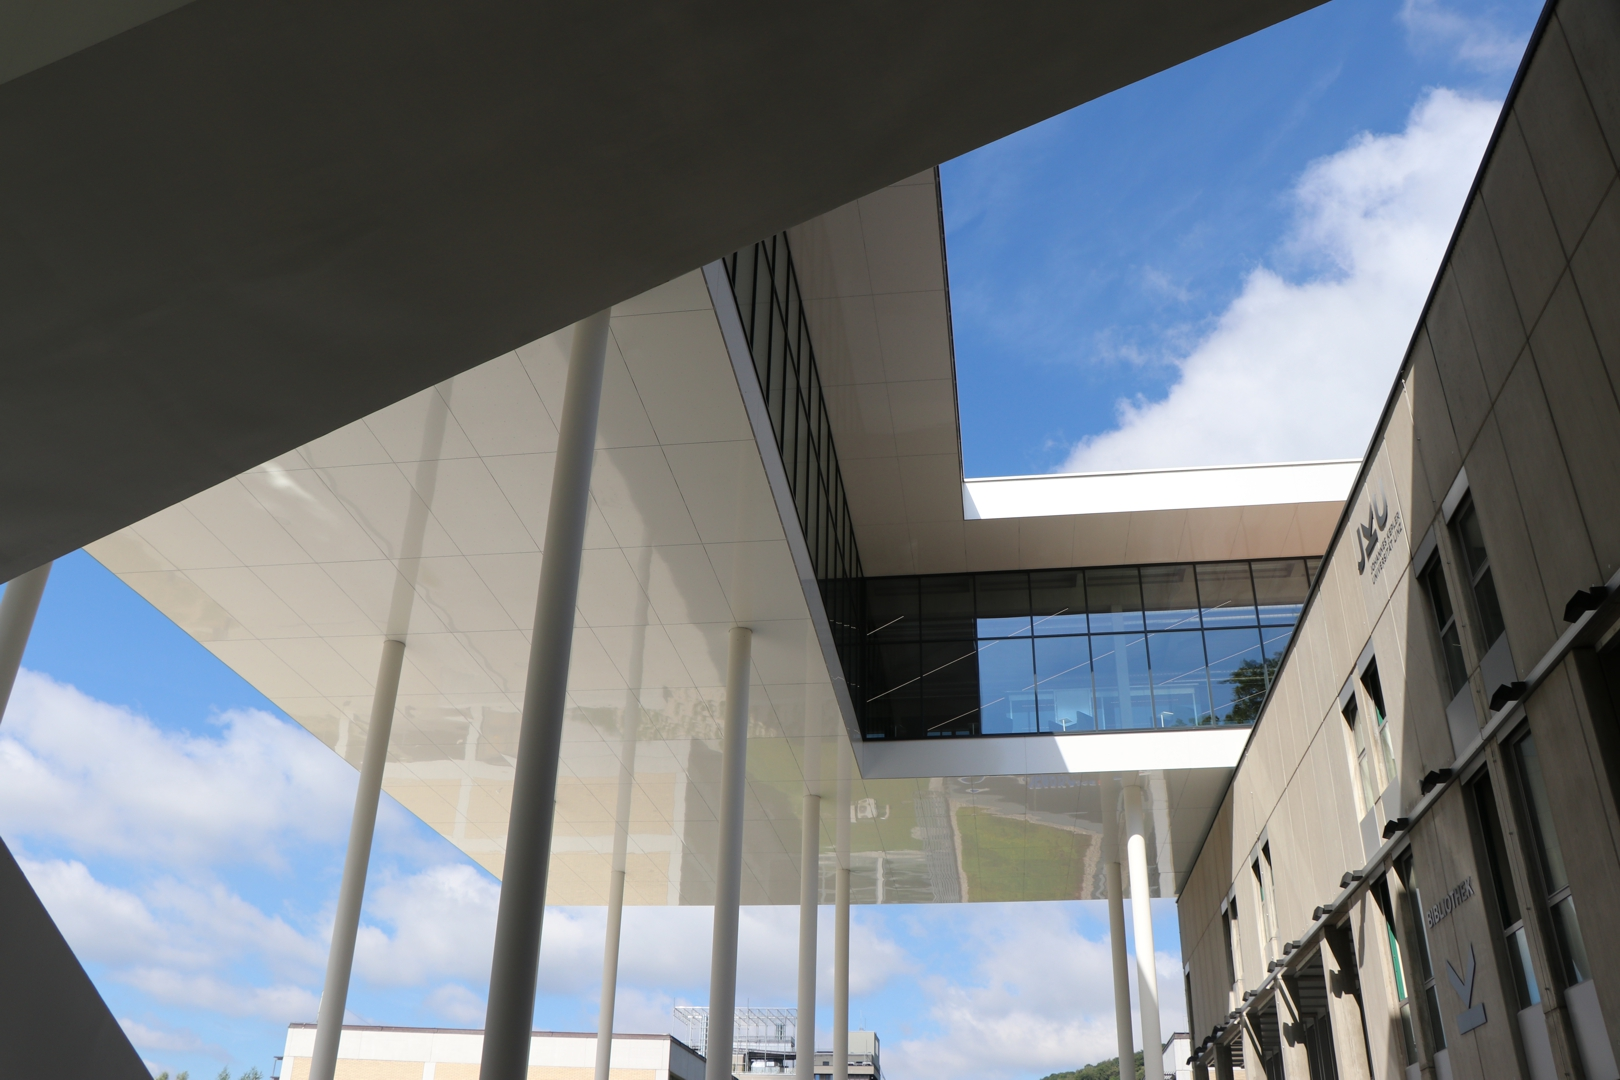
\includegraphics[width=\linewidth]{images/jku_learningcenter}
	\caption{
		A figure. Be aware that figures have their caption below the artwork
	}\label{fig:learningcenter}
\end{figure}
\begin{table}[t]
	\centering
	\caption{
		A table. Be aware that tables have their caption above the table
	}\label{tab:nicetable}
	\begin{tabularx}{\linewidth}{l>{\raggedright\arraybackslash}X}
		\toprule
		\textbf{Option}        & \textbf{Description} \\
		\midrule
		\texttt{phdthesis}     & PhD thesis           \\
		\texttt{mathesis}      & Master's thesis      \\
		\texttt{diplomathesis} & Diploma thesis       \\
		\texttt{bathesis}      & Bachelor's thesis    \\
		\texttt{seminarreport} & Seminar report       \\
		\texttt{techreport}    & Technical report     \\
		\bottomrule
	\end{tabularx}
\end{table}

You will often reference and quote other works.
With \texttt{natbib}, there are different ways to cite the work of others.
These are a few examples using the updated bibliography keys:

\begin{itemize}
	\item Recent advances in reinforcement learning have significantly improved reasoning capabilities \citep{laser}. Be aware that the \texttt{\textbackslash citep} command puts the citation in parentheses.
	\item \citet{r1} demonstrate how incentivizing reasoning capability can be achieved via reinforcement learning. Here we used \texttt{\textbackslash citet} for a textual citation.
	\item \citet{verifystepbystep} emphasize the importance of verifying steps individually to improve model reliability.
	\item Several studies have pushed the limits of mathematical reasoning in language models \citep{deepseekmath, deepmath103k}. Note that multiple citations are separated by semicolons in this style.
	\item \citet{laser} conclude:
	      \begin{quote}
		      \emph{By mathematically equating the optimal verifier reward to the last-token self-rewarding score, the authors enable models to learn reasoning and verification jointly.}
	      \end{quote}
\end{itemize}


\section{Conclusion}
\label{sec:conclusion}

Space for your summary, central conclusions, and an outlook on potential future work.


%%
%%%%%%%%%%%%%%%%%%%%%%%%%%%%%%%%%%%%%%%%%%%%%%%%%%%%%%%%%%%%%%%%%%%%%%%%%%%%%%%%

%%%%%%%%%%%%%%%%%%%%%%%%%%%%%%%%%%%%%%%%%%%%%%%%%%%%%%%%%%%%%%%%%%%%%%%%%%%%%%%%
%%
%% Print the bibliography
%%
\cleardoubleoddpage

%% Replaced \printbibliography with standard BibTeX commands
\bibliographystyle{plainnat}
\bibliography{references}

%%
%%%%%%%%%%%%%%%%%%%%%%%%%%%%%%%%%%%%%%%%%%%%%%%%%%%%%%%%%%%%%%%%%%%%%%%%%%%%%%%%

%% Begin with the appendix part (all further sections will be appendices)
\appendix

\section{An Appendix}
\label{app:an-appendix}

Space for an appendix.


\cleardoubleoddpage

\end{document}